\documentclass{beamer}

\title{Stock Picking \& Structural Breaks}

\author{Jeppe Søndergaard Johansen (pcv439)}

\usetheme{Frankfurt}
\usecolortheme{orchid}


%additional usepackages
\usepackage{amsmath}
\usepackage{tikz}
\usepackage{ amssymb }
\usepackage{import}
\usepackage[ruled,vlined]{algorithm2e}
\usepackage{booktabs}
\usepackage[capposition=top]{floatrow}
\usepackage{scrextend}
\usepackage{csquotes}
\usepackage{graphicx}

%new commands
\newcommand{\ances}{AN_{A}^{\mathcal{G}}}
\newcommand{\anc}{\mathbf{AN}^{\mathcal{G}}}
\newcommand{\dec}{\mathbf{DE}^{\mathcal{G}}}
\newcommand{\dsep}{\text{ \textit{d}-sep }}
\newcommand{\dseperation}{\text{ \textit{d}-seperation}}
\newcommand{\nodes}{\mathbf{V}}
\newcommand{\parents}{\mathbf{PA}^{\mathcal{G}}}
\newcommand{\parentsNew}{\mathbf{PA}^{\mathcal{G^{*}}}}
\newcommand{\summ}{\frac{1}{n}\sum_{i=1}^{n}}


\newcommand{\children}{\mathbf{CH}^{\mathcal{G}}}

\newcommand{\graph}{\mathfrak{C}}
\newcommand{\E}{\mathbb{E}}
\newcommand{\std}{\mathbf{std}}
\newcommand{\R}{\mathbb{R}}
\newcommand{\G}{\mathcal{G}}
\newcommand{\lra}{\Leftrightarrow}

\newcommand{\la}{\leftarrow}
\newcommand{\ra}{\rightarrow}

\newcommand{\rp}{\right)}
\newcommand{\lp}{\left(}

%%%% INDEPDENT SIGN %%%%

\makeatletter
% Taken from http://ctan.org/pkg/centernot
\newcommand*{\centernot}{%
  \mathpalette\@centernot
}
\def\@centernot#1#2{%
  \mathrel{%
    \rlap{%
      \settowidth\dimen@{$\m@th#1{#2}$}%
      \kern.5\dimen@
      \settowidth\dimen@{$\m@th#1=$}%
      \kern-.5\dimen@
      $\m@th#1\not$%
    }%
    {#2}%
  }%
}
\makeatother

\newcommand{\independent}{\perp\mkern-9.5mu\perp}
\newcommand{\notindependent}{\centernot{\independent}}

%%%%% INDEPENDENT SIGN END %%%%%

\newcommand{\X}{\mathbf{X}}
\newcommand{\Ls}{\mathbf{L}}
\newcommand{\D}{\mathbf{D}}
\newcommand{\W}{\mathbf{W}}

\newcommand{\x}{\mathbf{x}}
\newcommand{\ls}{\mathbf{l}}
\newcommand{\ds}{\mathbf{d}}
\newcommand{\w}{\mathbf{w}}

\newcommand{\rr}{\mathbf{r}}
\newcommand{\RR}{\mathbf{R}}

\newcommand{\ones}{\mathbf{1}}

\DeclareMathOperator*{\argmax}{arg\,max}
\DeclareMathOperator*{\argmin}{arg\,min}


\begin{document}



\maketitle

\begin{frame}
\tableofcontents
\end{frame}

\begin{frame}
\frametitle{Introduction \& Overview}

This paper investigates strategies for stock picking, where stock picking is assumed to be at any period only having a single stock, in an environment of structural breaks. The investigation follows the structure of:
\begin{enumerate}
    \item Model outline.
    \item A description of data.
    \item Model identification and fitting the parameters. A data set is simulated using these results.
    \item An ensemble of algorithms are discussed, and the best performing algorithm is found using the simulated data set.
    \item The best performing algorithm is applied on the real data set, and compared to a set of benchmarks.
\end{enumerate}

\end{frame}


\section{Model}

\begin{frame}
\frametitle{DGP in classic CAPM}

\begin{itemize}
    \item Returns are assumed to follow a DGP with constant covariance matrix and expected returns
    \item In this application i've restricted the assumption s.t. the returns are normally distributed.
\end{itemize}

\begin{equation}
    \RR^{(t)} \sim N(\mu, \Omega)
\end{equation}

\end{frame}

\begin{frame}
\frametitle{DGP under assumptions of structural breaks}

\begin{itemize}
\item I modify the assumption, and say at any point in time a structural break can occur.
\item A structural break implies a new covariance matrix and vector of expected returns are drawn
\end{itemize}

\begin{equation}\label{eq:structuralbreak}
    b^{(t)} = bern(p)
\end{equation}

\begin{equation}
    \mu^{(t)} \sim d_{\mu} \qquad \Omega^{(t)} \sim d_{\Omega}, \qquad \text{if $b=1$}
\end{equation}

\begin{equation}
    \mu^{(t)} = \mu^{(t-1)} \qquad \Omega^{(t)} = \Omega^{(t-1)}, \qquad \text{if $b=0$}
\end{equation}

\begin{equation}
    \RR^{(t)} \sim N(\mu^{(t)}, \Omega^{(t)})
\end{equation}

\end{frame}

\section{Data}

\begin{frame}
\frametitle{Data}

\begin{itemize}
    \item The data consists of 11 stocks for approximately 30 years ($\approx 7000$ observations).
    \item The data is acquired through a public API provided by \textbf{Quandle}.
    \item The individual stocks represents a wide variety of companies from different sectors.
    \item To get stationarity in the data, the data is transformed by:
    \begin{equation}
            r_{i}^{(t)} = \frac{a_{i}^{(t)}}{a_i^{(t-1) }}   - 1
    \end{equation}
    \item The risk free asset is assumed to be of $2 \%$ annually throughout the paper.
\end{itemize}

\end{frame}

\begin{frame}
\frametitle{Historical traces}

\centering
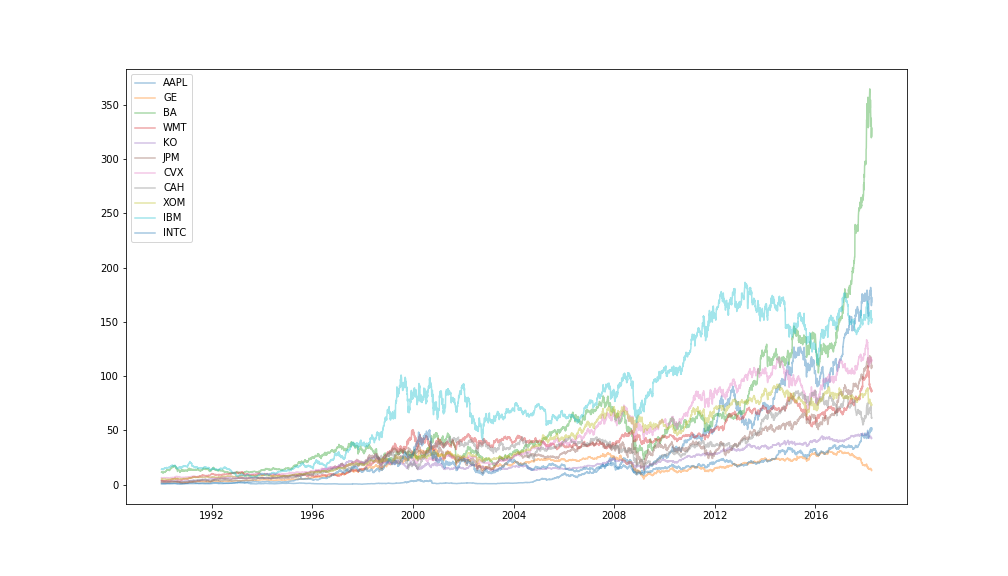
\includegraphics[scale=0.32]{../figures/historicaltraces.png}

\end{frame}

\begin{frame}
\frametitle{Summary statistics of Stocks}
\centering
\resizebox{\columnwidth}{!}{%
\begin{tabular}{lrrrrrrrrrrr}
\toprule
{} &    AAPL &      GE &      BA &     WMT &      KO &     JPM &     CVX &     CAH &     XOM &     IBM &    INTC \\
\midrule
mean &  0.0011 &  0.0004 &  0.0006 &  0.0006 &  0.0005 &  0.0008 &  0.0005 &  0.0007 &  0.0005 &  0.0005 &  0.0009 \\
std  &  0.0282 &  0.0175 &  0.0187 &  0.0165 &  0.0141 &  0.0241 &  0.0153 &  0.0188 &  0.0145 &  0.0174 &  0.0240 \\
min  & -0.5187 & -0.1279 & -0.1763 & -0.1018 & -0.1047 & -0.2073 & -0.1249 & -0.2454 & -0.1395 & -0.1554 & -0.2202 \\
25\%  & -0.0128 & -0.0079 & -0.0092 & -0.0079 & -0.0064 & -0.0101 & -0.0078 & -0.0084 & -0.0072 & -0.0079 & -0.0115 \\
50\%  &  0.0001 &  0.0000 &  0.0001 &  0.0000 &  0.0000 &  0.0000 &  0.0002 &  0.0000 &  0.0000 &  0.0001 &  0.0004 \\
75\%  &  0.0144 &  0.0087 &  0.0104 &  0.0087 &  0.0072 &  0.0107 &  0.0089 &  0.0097 &  0.0082 &  0.0087 &  0.0130 \\
max  &  0.3322 &  0.1970 &  0.1546 &  0.1107 &  0.1388 &  0.2510 &  0.2085 &  0.2039 &  0.1719 &  0.1316 &  0.2012 \\
\bottomrule
\end{tabular}

}

\end{frame}


\begin{frame}
\frametitle{Structural Breaks (Visual inspection)}

\centering
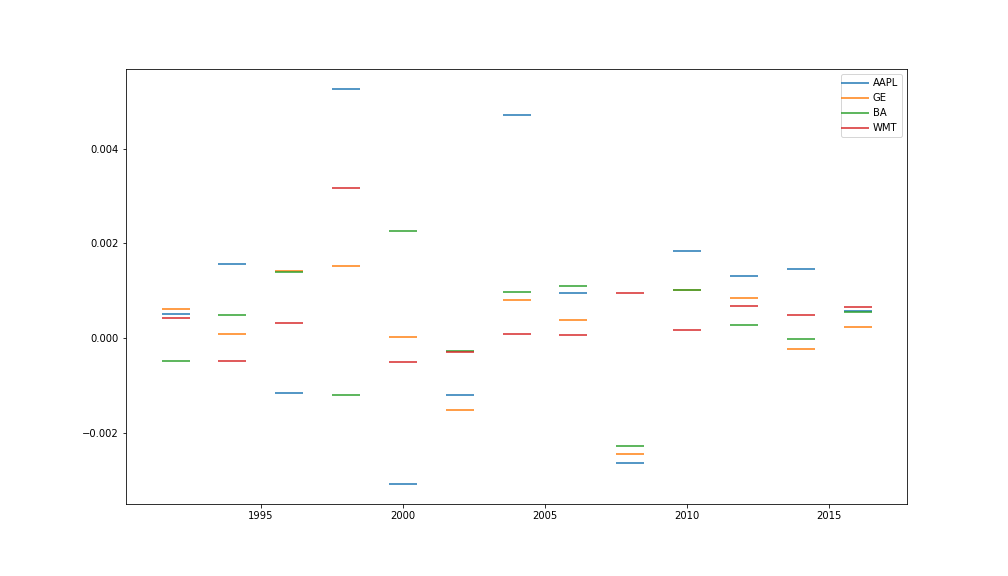
\includegraphics[scale=0.32]{../figures/structural_breaks_means.png}

\end{frame}

\section{Fitting the model}

\begin{frame}
\frametitle{Identification strategy}
\begin{itemize}
    \item Sampling from the structural model, requires the distributions to be specified, and the parameters of the distributions to be estimated.
    \item The $d_{\mu}$ is assumed to be normal, and $d_{\Omega}$ is found by a transformation of variances and correlations.
    \item the variances is assumed to be exponentially distributed, and the correlations is assumed to be normally distributed.
    \item When the model is identified, $11 \times 2.000.000$ observations are simulated. This data set can be used to training and tuning different algorithms on.
\end{itemize}

\end{frame}

\begin{frame}
\frametitle{Distribution of Returns, $d_{\mu}$}

\centering
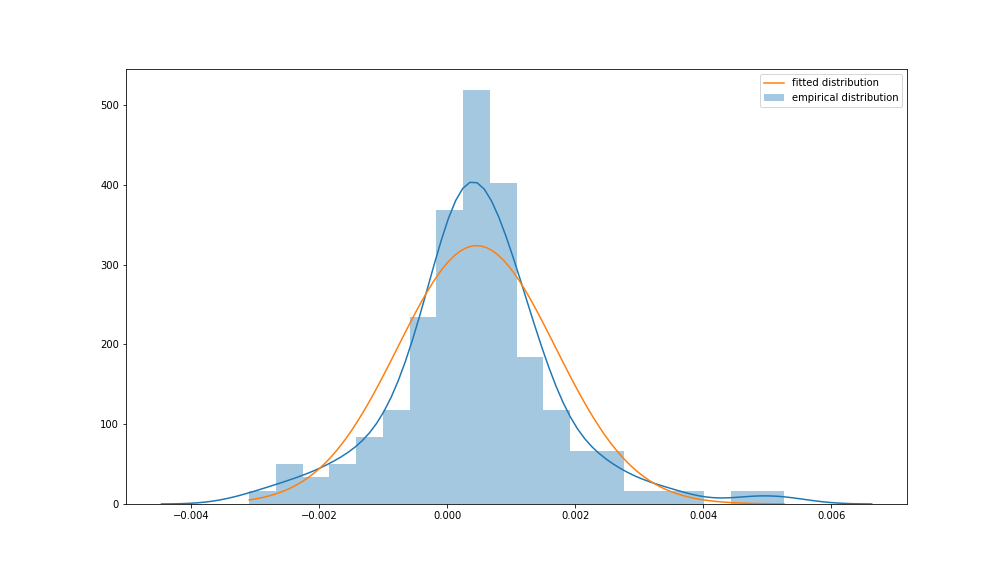
\includegraphics[scale=0.32]{../figures/distribution_means.png}

\end{frame}

\begin{frame}
\frametitle{Distribution of Variances, $\sigma_i^{2}$}

Needing to sample the covariance matrix, I find the distribution og variances, and the correlation matrix.

\centering
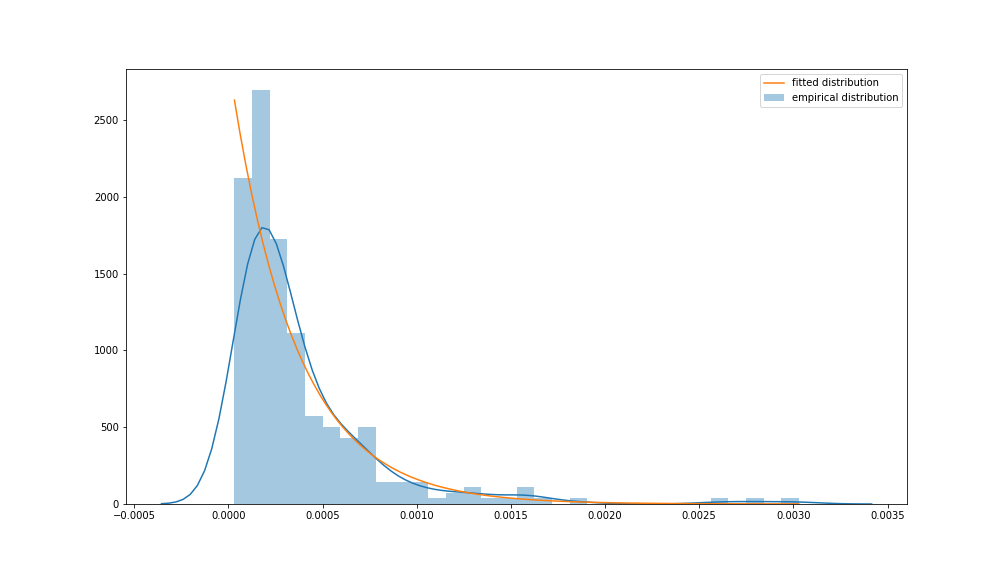
\includegraphics[scale=0.32]{../figures/distribution_variances.png}

\end{frame}


\begin{frame}
\frametitle{Distribution of individual correlations, $\rho_{i,j}$}

\centering
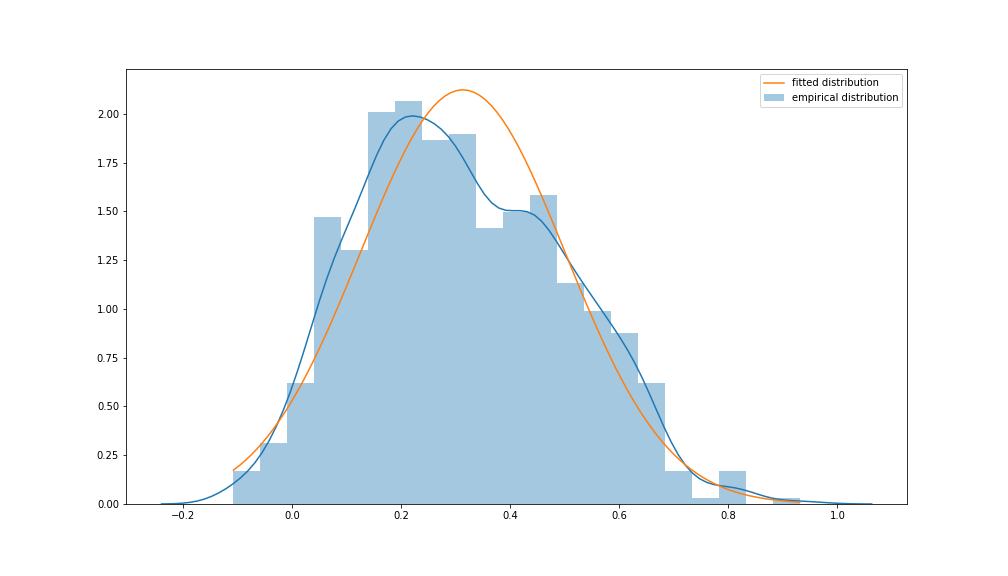
\includegraphics[scale=0.32]{../figures/correlation_distribution.png}

\end{frame}

\begin{frame}
\frametitle{Simulated Covariances vs. Empirical Covariances, $\sigma_{i,j}$}

\centering
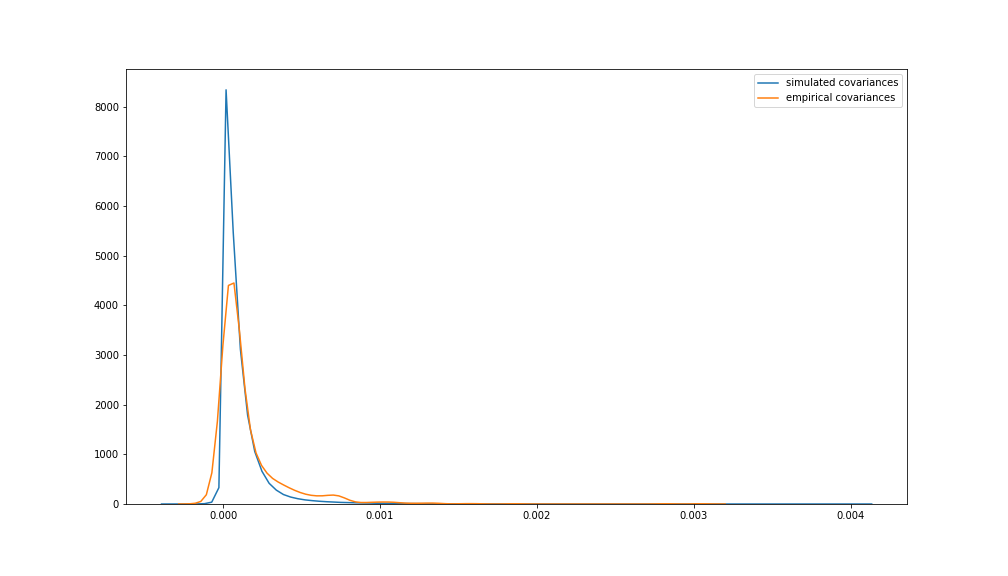
\includegraphics[scale=0.32]{../figures/dist_simulated_covariances.png}

\end{frame}

\section{Algorithms}

\begin{frame}
\frametitle{Overview of 3 algorithms}
\begin{itemize}
    \item \textbf{LSTM}: Neural network based algorithm used for patern representation in time series problems. Used in self driving cars, and state of the art chess computers.
    \item \textbf{Naive Rolling Sharpe} Use the rolling Sharpe ratios on the different stock to pich the stock with highest sharpe ratio
    \item \textbf{Rolling Sharpe} An extension of the algorithm above, but with the capability to forget its distant past.
\end{itemize}
\end{frame}

\begin{frame}
\frametitle{Strategy for algorithm selection}
\begin{itemize}
    \item The three algorithms are tested on the simulated data set. The best performing algorithm (lowest \textit{mean squared error}) is used on the real data set.
    \item Since the true variance and std. deviations in the simulated dataset are known the true Sharpe ratio can be calculated for each simulated stock in each time step.
    \item The \textit{mean squared error} is found between the true Sharpe ratio and the Sharpe ratio predicted by the algorithm.
    \item The best performing algorithm is found to be \textbf{Rolling Sharpe}
\end{itemize}

\end{frame}


\begin{frame}
\frametitle{Predicted vs. actual Sharpe ratios}

\centering
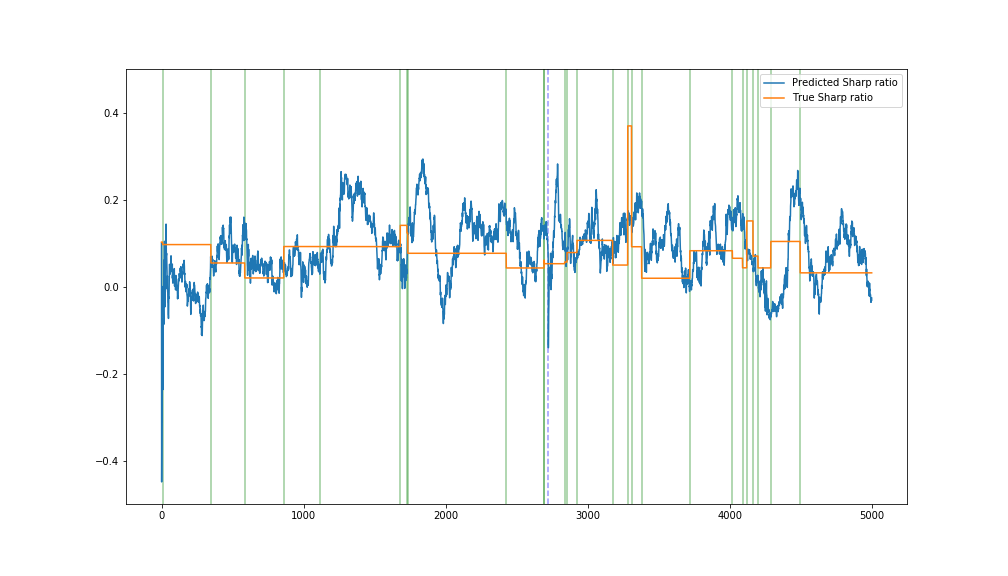
\includegraphics[scale=0.32]{../figures/rolling_sharp_prediction_simulated.png}


\end{frame}



\section{Analysis}

\begin{frame}
\frametitle{Analysis}

\begin{itemize}
\item Taking the \textbf{Rolling Sharpe} algorithm to the real data we need benchmarks.
\item 4 benchmarks is used: 1) The \textit{Apple} stock, 2) The tangency portfolio calculated on the first 1000 observations, 3) The tangency portfolio calculated on the entire sample, 4) Perfect foresight.
\end{itemize}

\end{frame}

\begin{frame}
\frametitle{Performance Comparison (part 1)}

\centering
\resizebox{\columnwidth}{!}{%
\begin{tabular}{lrrr}
\toprule
{} &  Expected Return &      Std &  Sharpe Ratio \\
\midrule
rolling sharpe                &          0.00263 &  0.02028 &       0.12562 \\
perfect stock pick            &          0.02515 &  0.02285 &       1.09734 \\
apple                         &          0.00111 &  0.02824 &       0.03661 \\
tangency portfolio (1000 obs) &          0.00058 &  0.01830 &       0.02719 \\
tangency portfolio (all obs)  &          0.00077 &  0.01246 &       0.05545 \\
\bottomrule
\end{tabular}

}

\end{frame}


\begin{frame}
\frametitle{Performance Comparison (part 2)}

Counterfactual portfolios, using different strategies

\centering
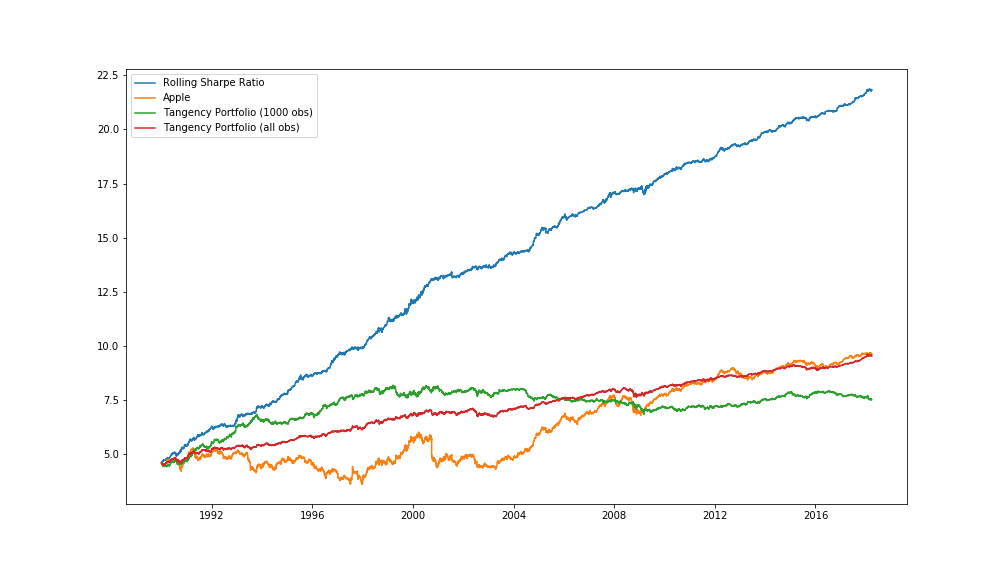
\includegraphics[scale=0.32]{../figures/log_investment_experiment.png}

\end{frame}

\begin{frame}
\frametitle{Performance Comparison (part 3)}

Monte carlo simulation, using moments of portfolios from real data.

\centering
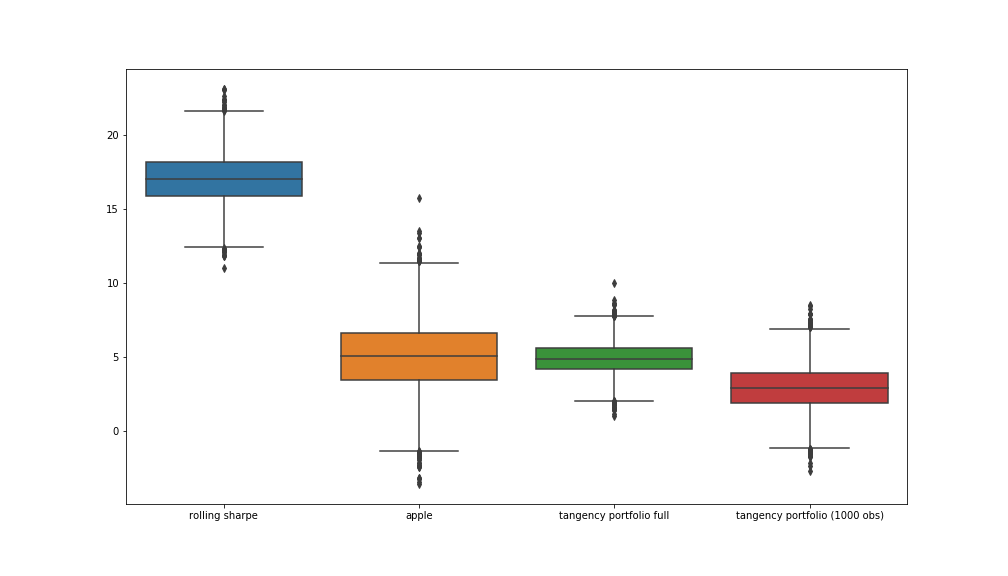
\includegraphics[scale=0.32]{../figures/boxplot_monte_carlo.png}

\end{frame}


\section{Conclusion \& Discussion}

\end{document}
